
% ========== Chapter 2
 
\chapter {Charge Collection and Surface Effects in HPGe Detectors}\label{ch:HPGe_det}
\section{HPGe Detector Basics}
High-purity Germanium (HPGe) detectors are made from one large semiconductor crystal of low impurity-concentration germanium, forming a diode (i.e. p-n junction). Two electrical contacts, the p$^+$ and n$^+$ contacts, are made on the crystal's surface, and the entire crystal is reverse-biased, resulting in a depleted region between the contacts. When the detector is biased to its operating voltage (generally between 1 and 5\,kV), its entire volume is fully depleted, and the charge drift speeds in the interior are fully saturated. In other words, applying a higher bias voltage will not change the current produced at the contacts. The electric field (and therefore, the pattern of charge drift paths) in the interior of the detector is fixed, set by the shape of the electrical contacts at the surface and, in some cases, the doping of the crystal. 

In normal operation, currents in the detector are produced when some form of radiation penetrates the active volume, moving electrons in the crystal from the valence band to the conduction band. This leaves a vacancy in the valence band called a ``hole," which behaves as a positive charge in the electric field. The amount of energy needed to create such an ``electron-hole pair" depends on the size of the band gap in the crystal. 

In germanium, the band gap is very small, at 0.7\,eV \cite{Bertolini1968}. Therefore, thermal excitations at room temperature can easily create electron-hole pairs. To reduce this ``dark current," the detector must be cooled, generally to between 77 and 100\,K using liquid nitrogen. The main advantage of semiconductor detectors like HPGe detectors is in the small amount of energy needed to create an electron-hole pair. In Ge at 77\,K, only 2.96\,eV is needed for each pair. This gives the detectors intrinsically high resolution, or at least, the potential for high resolution. 

Once in the conduction band, the electrons and holes drift to the n$^+$ and p$^+$ contacts, respectively, inducing a current on the contacts. The integral of the current induced on either contact is proportional to the energy of the interaction that originally created the cloud of electron-hole pairs. Currents from both charge carriers sum to give the observed signal; the fraction contributed by each type of carrier depends on position of origin of the charges and the electric field, which in turn depends on the doping of the detector. 

\begin{figure}[]
 \centering
 \includegraphics[height = 3in]{/Users/jgruszko/Documents/Thesis/Images/Ch2/HPGe_types.png}
 \caption[$p$- and $n$-type HPGe detectors]{Diagrams of coaxial detector cross-sections for $p$- \textit{(left)} and $n$- \textit{(right)} type HPGe detectors. From \cite{KnollText}.} 
 \label{fig:Ge_types}

 \centering
 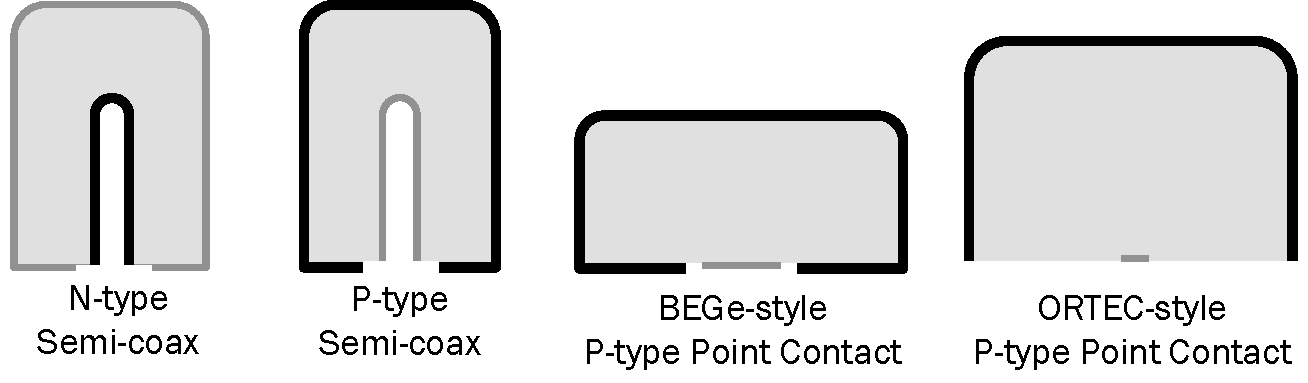
\includegraphics[width = \textwidth]{/Users/jgruszko/Documents/Thesis/Images/Ch2/det_types.pdf}
 \caption[Various geometries of HPGe detectors]{Cartoon showing the geometries and electrode arrangements of semi-coaxial and point-contact detectors. The black line indicates the n$^+$ contact, the grey line is the p$^+$ contact, and the gap in the outline indicates passivation to create an insulating surface. Dimensions not to scale.} 
 \label{fig:det_types}
\end{figure}

HPGe detectors are made in $p$- and $n$-types, determined by their doping. $n$-type detectors are doped with electron donor impurities, so called because they leave one loosely-held valence electron available after bonding to the surrounding Ge atoms. The net effect of these impurities, even at low doses, is to give an excess of conduction electrons and a deficit of holes compared to the un-doped material. This means that for almost all charge origin positions in $n$-type detectors the majority of the observed current is made by the electrons, with a small contribution from the holes. To take advantage of this fact, $n$-type detectors have their electrical contacts arranged as in Figs.~\ref{fig:Ge_types} and \ref{fig:det_types}, with the geometry giving a large field gradient near the n$^+$ contact, where the signal is read out. 

The reverse is true of $p$-type detectors, which are doped with electron acceptor impurities. In this case, the holes provide most of the current, and the signal is read out at the p$^+$ contact. 

\begin{SCfigure}[]
 \centering
 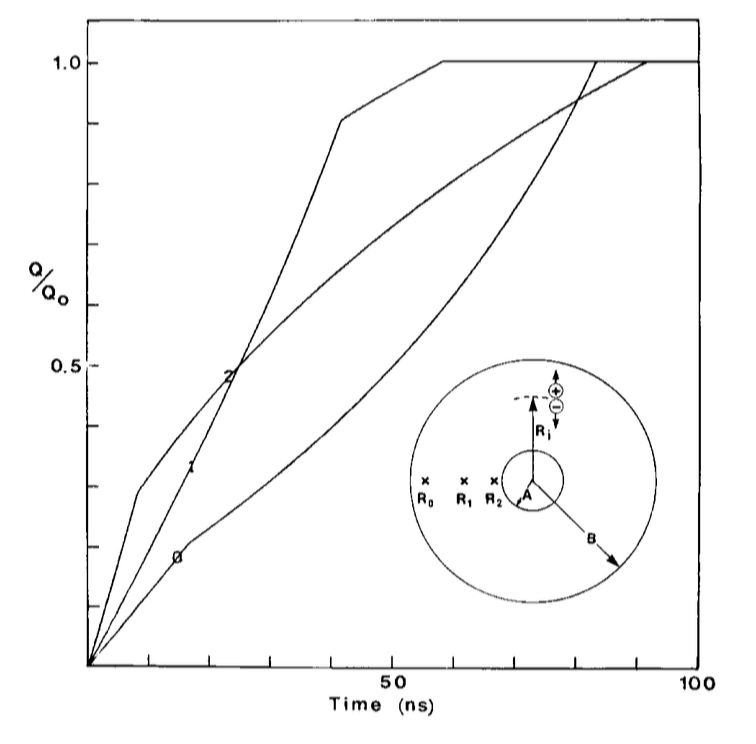
\includegraphics[height = 3in]{/Users/jgruszko/Documents/Thesis/Images/Ch2/n_sim_sig.png}
 \caption[Calculated signals in an $n$-type Ge(Li) detector]{Calculated pulse shapes for several interaction positions in an $n$-type Ge(Li) detector. Three different interactions points are indicated as 0, 1, and 2. From \cite{Gadeken1976}.} 
 \label{fig:n_sim}
\end{SCfigure}

\begin{SCfigure}[]
 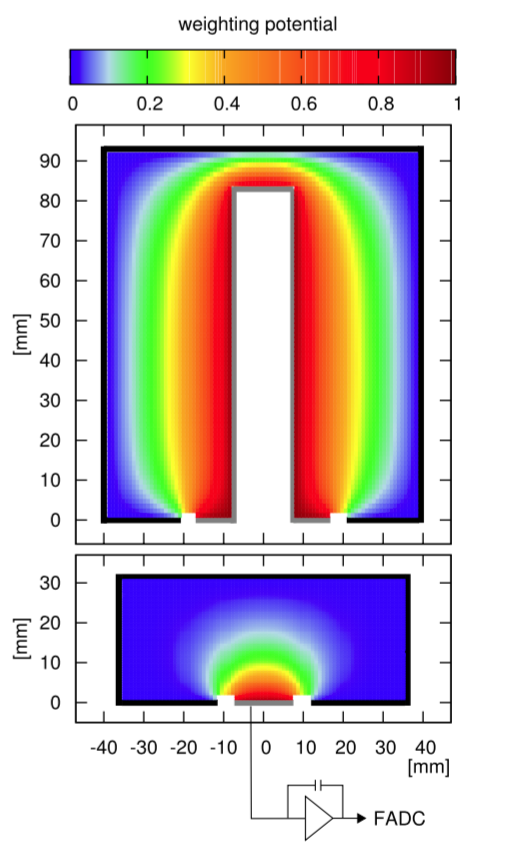
\includegraphics[width = .40\textwidth]{/Users/jgruszko/Documents/Thesis/Images/Ch2/wp_GERDA.png}
 \caption[Weighting potential maps of a coaxial and BEGe-type detector]{Cross section of a $p$-type semi-coaxial detector \textit{(top)} and a $p$-type BEGe-style point contact detector \textit{(bottom)}. The p$^+$ contact is drawn in grey, with the n$^+$ contact in black. The gap between the contacts is an insulating passivated groove. The BEGe is shown with a charge sensitive amplifier like the LMFEs used to read out the \MJ\ detectors. Image from \cite{Agostini2013}.} 
 \label{fig:wp_all}
\end{SCfigure}

In both types of detectors, the fractional contribution of the two types of carriers also varies as a function of the event origin position (i.e. where in the volume of the crystal the charge cloud is created). In an $n$-type coaxial detector, as shown in Fig.~\ref{fig:n_sim}, signals from events near the central (n$^+$) contact, like event 2, will have a small fast electron-fraction, and a large slower hole fraction. Near the outer (P$^+$) contact (i.e. event 0), the reverse will be true, with the signal having a small fast hole fraction, and a large slower electron fraction. Event 1 occurs at a halfway position, where the effect of the detector doping dominates the carrier fractions. Since the detector shown is $n$-type, its signal has a large electron fraction, and a small slower hole fraction. In all three cases, the opposite behavior is seen in $p$-type detectors. 

The varying contributions of the carrier types with event position can be visualized in a weighting potential diagram, like those shown in Figs.~\ref{fig:wp_all} and \ref{fig:ppc_wp}. In Figs.~\ref{fig:wp_all} and ~\ref{fig:ppc_field}, an cross-section of the detector shows the fraction of the total signal contributed by the electrons as a function of radius $r$ and height $z$. In Fig.~\ref{fig:wp_z0}, the weighting potential is drawn as a function of $r$ at a chosen height (in this case, $z = 0$) in a $p$-type point-contact detector. As seen in these plots, signals in $p$-type detectors are dominated by the hole contribution over most of their volume. 

Until recently, large (1\,kg and above) HPGe detectors were made in semi-coaxial (seen in Fig.~\ref{fig:det_types}), coaxial, well, or segmented geometries. These designs ensured that no low-field regions, which lead to incomplete charge collection, remained in the corners of the detector. As seen in the upper image in Fig.~\ref{fig:wp_all}, these detectors have nearly constant weighting potential profiles at all heights. The drift path lengths of charge carriers from all positions in the crystal bulk are also similar. 

\begin{figure*}[t]
\centering
\begin{subfigure}[t]{.45\textwidth}
\centering
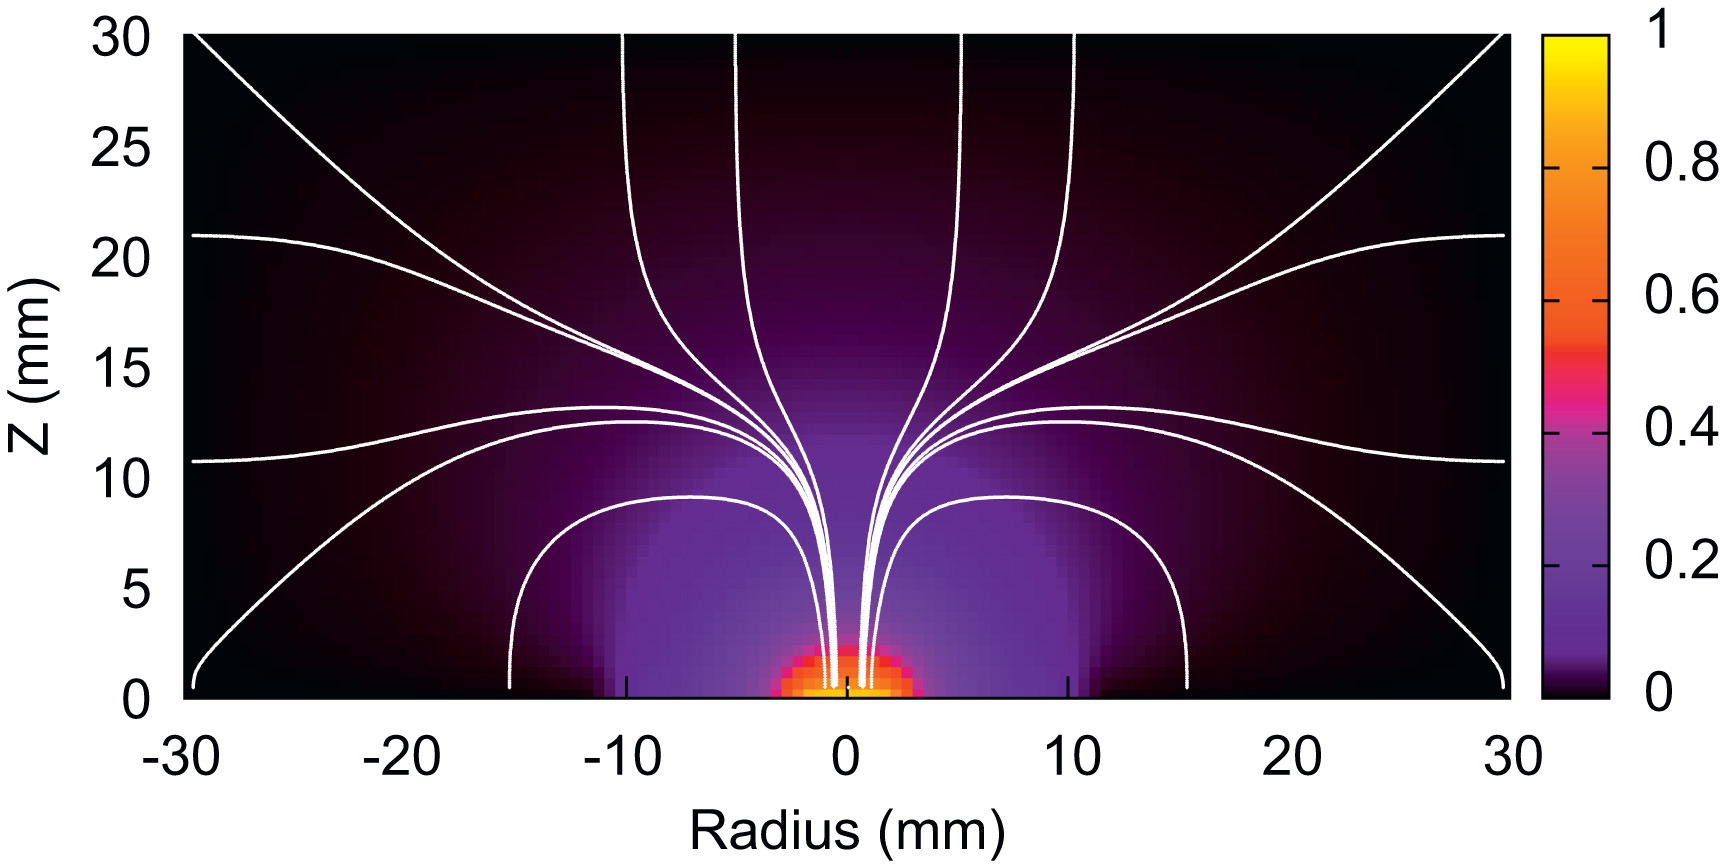
\includegraphics[width = \textwidth]{/Users/jgruszko/Documents/Thesis/Images/Ch1/PPCField.jpg}
\caption[Weighting potential map and drift paths of an ORTEC-type detector]{The charge drift paths (in white) are long and highly position-dependent. Image from \cite{Aalseth2011}.}
\label{fig:ppc_field}
\end{subfigure}
\hfil
\begin{subfigure}[t]{.45\textwidth}
\centering
 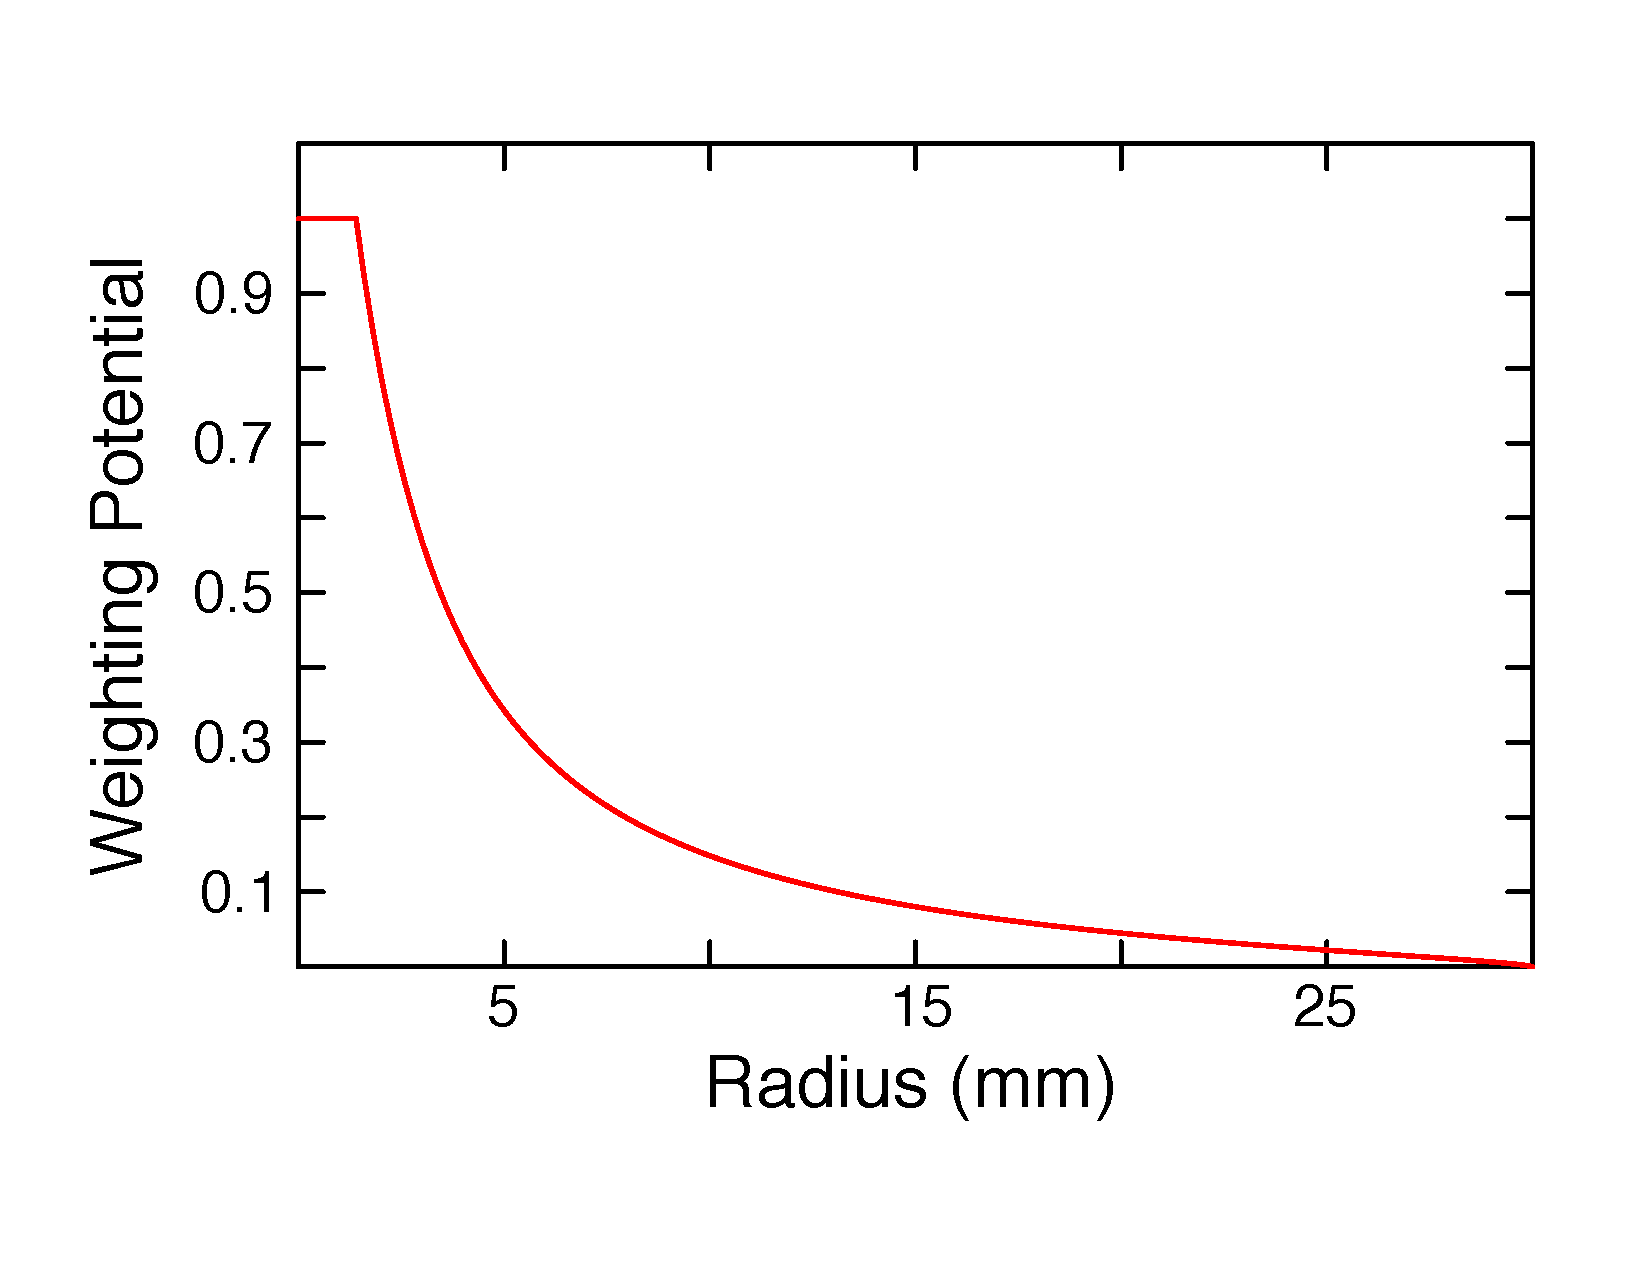
\includegraphics[width = \textwidth]{/Users/jgruszko/Documents/Thesis/Plots/Ch2/wp_z0}
 \caption[The weighting potential of a $p$-type point-contact detector]{The weighting potential at $z = 0$. Plot courtesy of David Radford.} 
 \label{fig:wp_z0}
 \end{subfigure}
 \caption{Simulations of the weighting potential in an $p$-type ORTEC-style point contact detector.}
  \label{fig:ppc_wp}
\end{figure*}


\section{P-Type Point Contact Germanium Detectors}
It has long been known that reducing the capacitance of HPGe detectors would reduce their noise and energy thresholds. This could done by using a small ``point-like" central contact, instead of the deep well used by coaxial detectors. The first attempts to make germanium detectors with point-contact geometries were made in 1989 by Luke et. al \cite{Luke1989}. Though these detectors had much smaller capacitance than coaxial detectors, they suffered from severe charge-trapping effects, degrading the detector resolution. 

The breakthrough improvement that made this geometry useful in 2007 came with the switch from $n$-type to $p$-type detectors. i.e., in switching from drifting electrons to drifting electron holes through the crystal \cite{Barbeau2007}. Since the holes are less susceptible to trapping, $p$-type point-contact (\ppc) detectors can achieve resolutions similar to those of coaxial detectors, with electric fields created primarily through careful control of the charge impurity gradient in the bulk of the crystal. 

Due to their geometry, \ppc s have capacitance of about 1\,pF, far lower than that of similarly-sized coaxial detectors. This leads to far lower noise than is found in coaxial detectors, and therefore lower thresholds. While \ppc s have masses up to 1\,kg, the thresholds that can be achieved are comparable to those of small ($\sim1$\,g) x-ray detectors \cite{Barbeau2007}. 

\subsection{Multi-site Pulse Shape Discrimination}
The most significant advantage of PPCs for $0\nu\beta\beta$ decay searches is in their pulse shape characteristics. Unlike in coaxial detectors, the distance that must be traveled by a charge cloud varies depending on where in the detector it is produced, as is clear in Fig.~\ref{fig:ppc_field}. Therefore, multi-site events, in which a $\gamma$ ray deposits energy at multiple points in the crystal, have clearly ``step-like" rise times, and can be identified and cut to reduce backgrounds. Double-beta decay, on the other hand, is intrinsically single-site since electrons have small mean free paths in germanium. Therefore the sacrifice of signal events in such an analysis is minimal. 

\begin{figure}[]
 \centering
 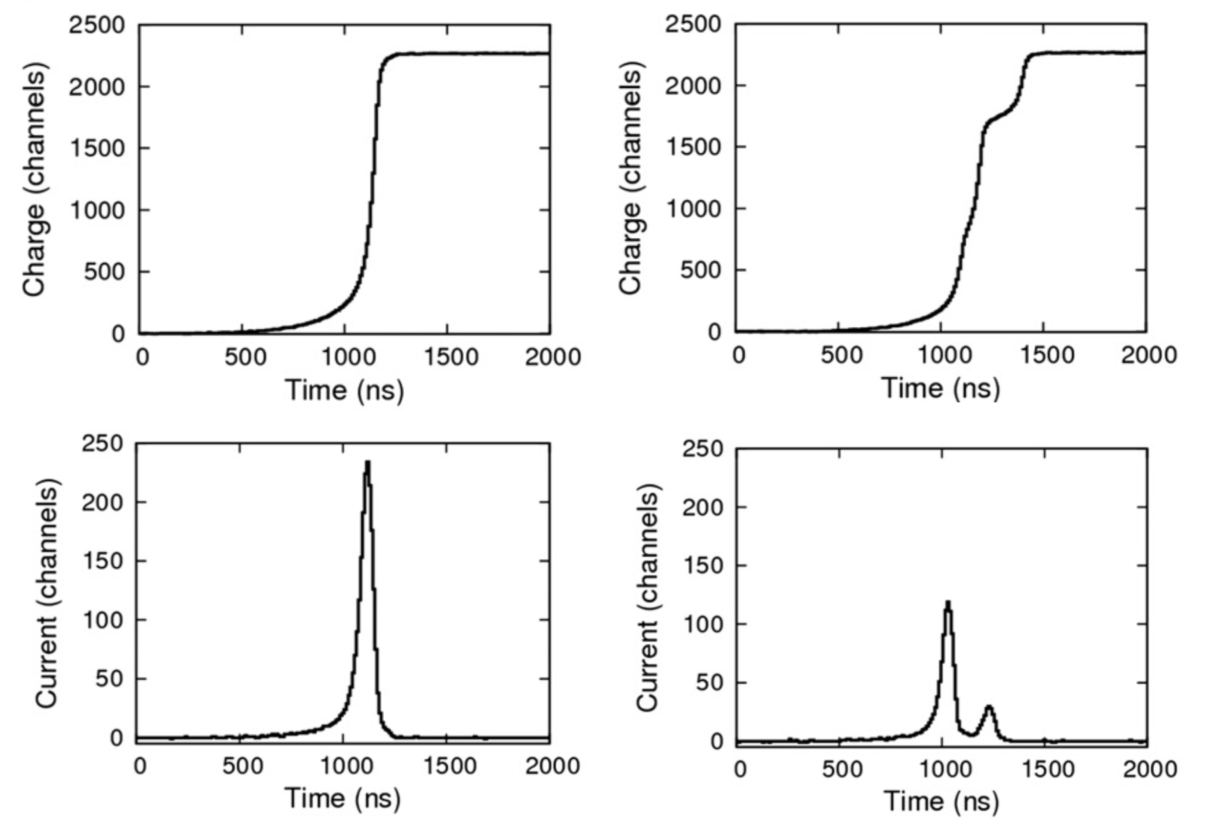
\includegraphics[width = .6\textwidth]{/Users/jgruszko/Documents/Thesis/Images/Ch2/ms_wf.pdf}
 \caption[Sample single- and multi-site waveforms in a \ppc\ detector]{Sample 1332\,keV single-site \textit{(left)} and multi-site \textit{(right)} waveforms in a \ppc\ detector. The charge read out from the detector \textit{(top)} shows the appearance of multiple steps in multi-site interactions, which leads to a reduced maximum current \textit{(bottom)} in these events. Image adapted from \cite{Cooper2011}} 
 \label{fig:PSD_wf}
\end{figure}%

As seen in Fig.~\ref{fig:PSD_wf}, one reliable way to identify these events is through the difference in their maximum current $A$. For a given energy $E$ of an event, which is proportional to the integral of the total current, multi-site events have lower-than-expected value of $A$. The pulse shape discrimination parameter used can be constructed from these parameters in a variety of ways. In this work, I use both their ratio $A/E$, with a correction for the energy dependence of $A$ \cite{Budjas2009} (called {\tt aenorm}), and the energy-corrected current ``A vs. E" (called {\tt avse})\cite{AvsE_unidoc}. 

The cut level in the parameter is set to accept 90\% of the $^{208}$Th double-escape peak, a sample of known single-site events, and reject events with {\tt aenorm} or {\tt avse} below the cut value. The effectiveness of the multi-site discrimination is evaluated by counting the remaining events in the single-escape peak (SEP), a sample of known multi-site events. Generally, the SEP and Compton continuum are reduced to approximately 10\% and 50\% of their original amplitudes, respectively.

Since the gamma backgrounds in the \nonubb\ ROI are dominated by Compton scattering events, the use of multi-site event discrimination in \ppc\ detectors provides a major increase in sensitivity. This is the main reason \ppc\ detectors were chosen by both the GERDA and \MJ\ Collaborations. 

\subsection{n$^+$ Surface Events}
Most of the surface of \ppc\ detectors is covered by the n$^+$ contact, a ruggedized layer of lithium that is diffused into the detector surface. Dedicated measurements have shown that this surface is characterized by two differently-behaving regions: a fully-dead conducting surface layer, in which there is no electric field and charge recombination occurs before the free charge carriers can enter the bulk, and a transition layer where incomplete charge collection occurs, and the energies of the observed events are degraded. Together, these have been measured to be 0.5 to 2\,mm thick, depending on the detector's fabrication techniques and thermal history. 

\begin{figure}[t]
 \centering
 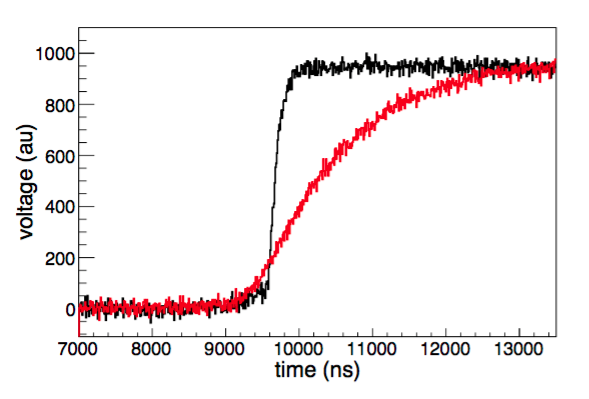
\includegraphics[height=2in]{/Users/jgruszko/Documents/Thesis/Images/Ch2/slowPulse.png}
 \caption[A sample n$^+$ slow pulse]{Sample bulk \textit{(black)} and n$^+$ \textit{(red)} surface events, both with energies of approximately 20\,keV, in the MALBEK \ppc\ detector. The n$^+$ surface event shows a distinctive slow pulse shape, with a 3\,$\mu$s rise-time, compared with bulk rise-times of 1 to 2 \,$\mu$s. Image from \cite{MALBEK2015}} 
 \label{fig:slowPulse}
\end{figure}

These measurements have also shown that events originating in the transition layer have a distinct ``slow-pulse" shape, with increased rise-time (and degraded values of $A$) compared to bulk events at the same energy. See Fig.~\ref{fig:slowPulse}. Based on simulations of charge transport, this is thought to be due to slow charge diffusion from the transition layer into the bulk \cite{MJD_slowpulses}. This process affects the entire rising edge of the pulse, slowing the rise time from the usual 1 to 2\,$\mu$s of events in the bulk of \ppc\ detectors, to approximately 3\,$\mu$s.  

\subsection{p$^+$ Surface Events}
The p$^+$ contact of a \ppc\ detector is formed by implanting boron ions into the surface, resulting in a contact that is 0.3\,$\mu$m thick. The size and shape of the p$^+$ contact region varies depending on the detector design. In BEGe-syle detectors, the contact has a radius of 5 to 6\,mm. In ORTEC-style detectors, the radius is 1.5 to 2\,mm.  

Events originating on or near the point-contact have distinct pulse shapes, with very fast rising edges and resulting anomalously high values of $A$. GERDA has therefore used an additional upper limit on $A/E$ to reject alpha events occurring on this surface \cite{GERDA2017}. Additional discussion of this approach is found in Ch.~\ref{ch:TUBE_analysis}. No charge trapping is expected in this region, and the only expected energy loss is due to the thin dead layer. 

\subsection{Passivated Surface Events}
The remainder of the detector surface is passivated, generally with GeO$_2$, to isolate the contacts from one another. In the BEGe-style design, the passivated area is limited to only the interior of the ``ditch" surrounding the point-contact, a toroidal groove less than 3\,mm in width. In the ORTEC-style detectors, the passivated area covers the entire bottom face of the cylindrical crystal, as shown in Fig.~\ref{fig:det_types}. 

The passivation layer itself is very thin, formed of just a few monolayers. Previous measurements, however, have shown that the charge collection in the passivated surface region is often incomplete, with high trapping observed in BEGe-type and segmented Ge detectors \cite{TUBE_GERDA} \cite{Abt2017}. Based on the data taken with the \MJ\ \DEM\ and simulations of charge transport on the surface \cite{Mullowney2012}, it was suspected that these events also featured distinctive pulse shapes caused by delayed charge collection. As further discussed in Ch~\ref{ch:DCR}, two potential processes were thought to drive the trapping and re-release: slow charge transport on the surface of the crystal, particularly of electrons, and bulk trapping and re-release at crystal dislocation sites near, but not on, the passivated surface. 

The effects observed near the passivated surface region are thought to depend on the technique used to passivate the surface and the electric field of the detector in that region, two factors that differ widely from one detector style and manufacturer to another. Therefore, it is key that the characteristics of these events be measured in each type of detector being used, particularly for ultra-low background experiments like GERDA and \MJ . 

\subsection{Bulk Charge-Trapping}
Charge-trapping in the bulk of the crystal, which causes low-energy tailing in gamma calibration peaks, has been observed in the \MJ\ \DEM. This trapping correlates linearly with drift time. The charge loss is of a constant fraction of the total charge in the event, meaning that it is also proportional to energy. This effect is corrected for in the \MJ\ analysis using an ``effective pole-zero correction" \cite{EnergyUnidoc}.

The rising edges of events with trapped charge are not noticeably affected, and the $A/E$ or $A vs. E$ of these events is normal. The charge trapping does, however, have a small but noticeable effect on our attempts to distinguish pulses from the passivated surface, as discussed in Ch.~\ref{ch:DCR}.

\section{Alpha Interactions in Ge}
\subsection{Alpha Energy Loss}
Alpha particles (i.e. $^4$He nuclei) primarily interact with matter through Coulomb interactions with the electrons of the absorber material. At high energies (above about 0.5\,MeV), their energy loss is described by the Bethe formula:
\begin{equation}
 -\frac{\mathrm{d}E}{\mathrm{d}x}  = \frac{4\pi e^4 z^2}{m_0 v^2} N B \\
 \end{equation}
 where 
 \begin{equation}
  B \equiv Z\left[ \ln \frac{2 m_0 v^2}{I} - \ln(1-\frac{v^2}{c^2}) - \frac{v^2}{c^2} \right]
   \end{equation}
$v$ and $ze$ are the velocity and charge of the primary particle, $N$ and $Z$ are the number density and atomic number of the absorber atoms, $m_0$ is the electron rest mass, and $e$ is the electron charge. The parameter $I$ is the average excitation and ionization potential of the absorber, and is experimentally determined \cite{KnollText}.

Using this formula, 5.0 to 5.5\,MeV alpha particles in germanium are expected to lose 215 to 205\,keV/$\mu$m. Their expected range is between 17.6 and 20.0\,$\mu$m. In copper, their expected range is between 10.1 and 11.5\,$\mu$m \cite{SRIM}. 
   
\subsection{Sources of Alpha Backgrounds}
Given the very low range of alpha particles in matter, any observed alpha backgrounds must originate within a line-of-sight of the sensitive detector surfaces. They may be from emitters on the detector surface itself, on the surfaces of parts near the detector, or from a very thin skin-depth of the materials' bulk. 

The most highly concerning source of alpha backgrounds in experiments like the \DEM\ is the decay of radon isotopes and their progeny, particularly $^{222}$Rn. Radon, a radioactive noble gas that is naturally created by the decay of uranium and thorium, is found in particularly high concentrations inside underground laboratories. Though many isotopes are created by the decays of $^{232}$Th and $^{238}$U, only $^{222}$Rn has a long-lived radioactive isotope in its subsequent decay chain. 

\begin{figure}[t]
 \centering
 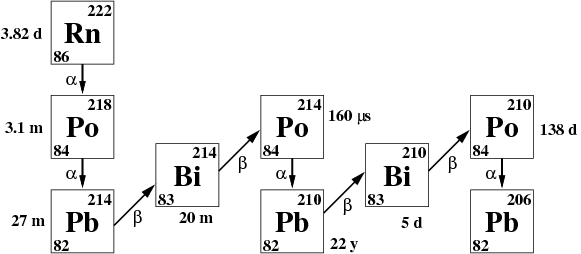
\includegraphics[height=2in]{/Users/jgruszko/Documents/Thesis/Images/Ch2/Rn222decay.png}
 \caption[The $^{222}$Rn decay chain]{The $^{222}$Rn decay chain, with the rare branchs to $^{218}$At and $^{210}$Tl removed for clarity. Image from \cite{Guiseppe2011}} 
 \label{fig:Rn222}
\end{figure}

Radon is particularly insidious in that as a noble gas, it easily permeates most materials. To reduce the impact of radon backgrounds, the \MJ\ Collaboration developed extensive cleaning procedures, particularly a method by which to surface-etch and passivate copper after machining \cite{Hoppe2007} that reduces the problem of $^{210}$Po re-deposition observed with other etching methods \cite{Zuzel2012}. Plastics were leached in nitric acid to reduce their surface contamination \cite{Overman2013}. 

Following cleaning, parts are stored and assembled under continuous nitrogen flow from liquid nitrogen boil-off, which is naturally low in radon. The resulting dry environment, however, can also lead to buildup of electrostatic charge, particularly on plastic parts. In its radioactive decay, radon creates charged progeny that can then be attracted to these surfaces. Deposition models are highly dependent on the environment, requiring dedicated studies in cleanroom and glovebox environments \cite{Guiseppe2011}. 

The $^{222}$Rn decay chain is pictured in Fig.~\ref{fig:Rn222}. The longest-lived isotopes are $^{210}$Pb, with a half-life of 22 years, and $^{210}$Po, with a half-life of 138 days. The short half-lives of all the isotopes occurring earlier in the chain imply that their decays are irrelevant to the backgrounds of the \DEM : as the experiment runs under vacuum and in a radon-purged environment, the short-lived isotopes from early in the decay chain will quickly decay, leading to a build-up of $^{210}$Pb. 

Of the subsequent decays, the most concerning is that of $^{210}$Po, which emits an alpha particle with 5.407\,MeV in 100\% of its decays. The other decays are either lower in energy than $Q_{\beta \beta}$, like the $\beta$ decays, or have very low branching ratios, like the alpha decay of $^{210}$Bi. The alpha decay of $^{210}$Po, on the other hand, can appear in the \nonubb\ ROI if its energy is degraded, whether by interactions in the material it is emitted from, by charge loss in dead regions of the detector, or by charge-trapping effects in the detector.  

This scenario, in which the parts or detectors are exposed to radon directly or to one of the isotopes falling between $^{222}$Rn and $^{210}$Pb in the decay chain, is called \textit{lead-supported} $^{210}$Po contamination. In this case, the 22\,yr half-life of $^{210}$Pb implies that the alpha background rate will remain constant over the life of the experiment. 

An alternative scenario, in which the chain is broken at $^{210}$Bi, can also occur. In this case, the rate of alpha background events will fall with the 138 day half-life of $^{210}$Po, leading to an improvement in the backgrounds over the life of the experiment. This is the case in the GERDA experiment \cite{GERDA_Background2013}. 

\subsection{Alpha Backgrounds in \ppc\ Detectors}
The small range of alpha particles in Ge implies, first of all, that all alpha events not originating inside the crystal itself should be considered potential ``surface events" in \ppc\ detectors. It also implies that the n$^+$ contact is entirely dead to alpha particles, and that alphas incident on the p$^+$ contact should be absorbed with energy loss of just 60\,keV. Therefore, alpha particles impinging on the n$^+$ surface will never pose a problematic background for \nonubb\ searches, and those on the p$^+$ surface will only contribute in the ROI if the alpha particle is emitted from the bulk of some material, and is therefore highly degraded before reaching the detector.

5.3\,MeV alphas incident on the passivated surface, on the other hand, could contribute to the backgrounds in the \nonubb\ ROI if there were significant energy degradation and/or charge trapping in this region. Indeed, as discussed in Ch.~\ref{ch:MJ_rates}, these decays appear to dominate the background rate of the \DEM\ above 2\,MeV. Therefore, an offline technique to reliably identify these events based on their pulse shape has been developed, as discussed in Ch.~\ref{ch:DCR}. 

To validate this technique, dedicated measurements were conducted of surface alpha events on the passivated surface of an ORTEC-style detector. These measurements and results are described in Ch.~\ref{ch:TUBE_exp} and Ch.~\ref{ch:TUBE_analysis}. These results can be used create a model for the charge loss in the passivated surface region that can subsequently be used in fits to the \MJ\ background spectrum. Analytic examples of this technique are used in Ch.~\ref{ch:MJ_rates} to estimate the position of the source of the alpha background events, and will be incorporated into full Monte-Carlo simulations of the \MJ\ backgrounds in future work. 

